
\chapter{Synchronous context free grammars} \label{sec:scfg}



\begin{figure}
\begin{center}
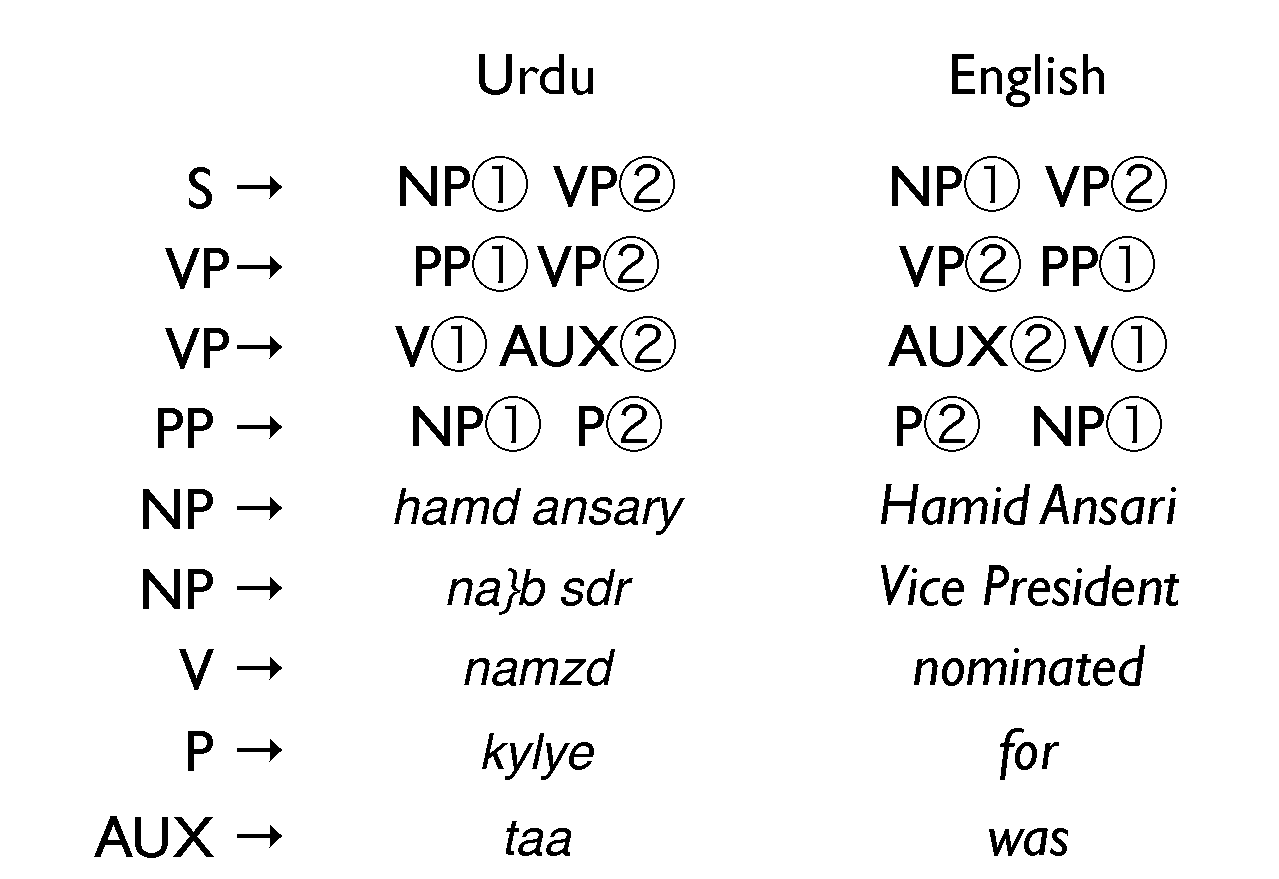
\includegraphics[width=.6\linewidth]{SCFGs/example-scfg}
\end{center}
\caption{A toy example that illustrates a SCFG that can translate (romanized) Urdu into English for one sentence.    }\label{toy-scfg} 
\end{figure}


\begin{figure}
\begin{tabular}{lll}
\multicolumn{3}{>{\columncolor[rgb]{0.95,0.95,0.75}}c}{The input is an Urdu sentence which is initially unanalyzed.}\\
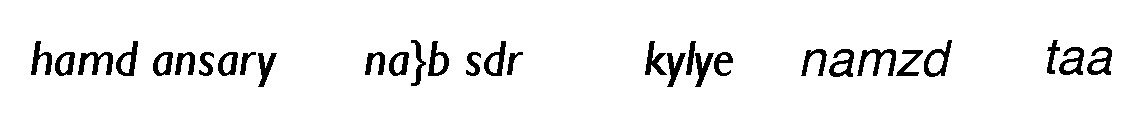
\includegraphics[width=.45\linewidth]{SCFGs/urdu-input} &  & 
\\ \hline
\multicolumn{3}{>{\columncolor[rgb]{0.95,0.95,0.75}}c}{Here all of the terminal symbols receive non-terminal labels.  The English words are in Urdu order.}\\
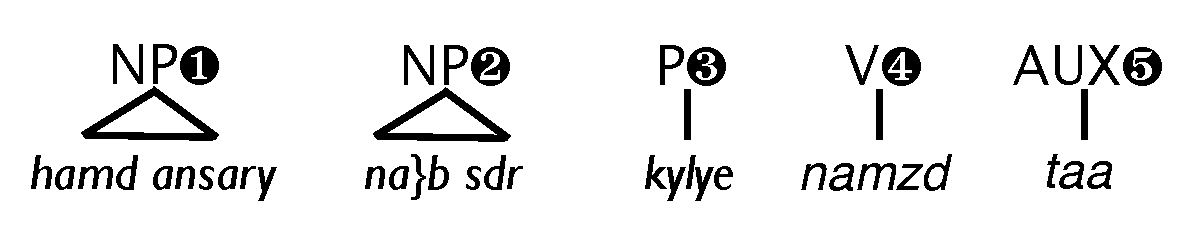
\includegraphics[width=.45\linewidth]{SCFGs/urdu-step0} & &
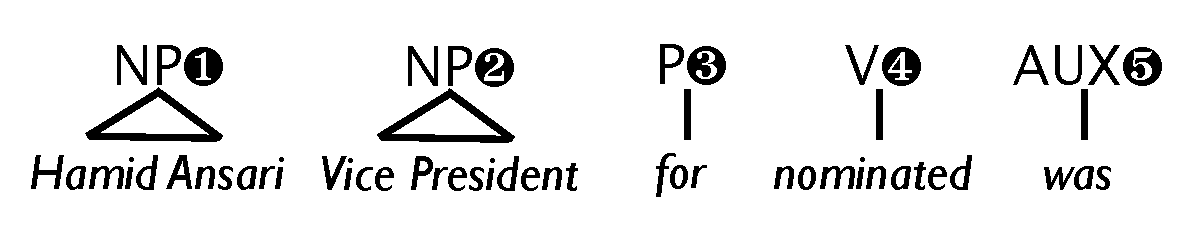
\includegraphics[width=.45\linewidth]{SCFGs/english-step0} \\ \hline
\multicolumn{3}{>{\columncolor[rgb]{0.95,0.95,0.75}}c}{The PP rule reorders the Urdu postpositional phrase to be a prepositional phrase on the English side.}\\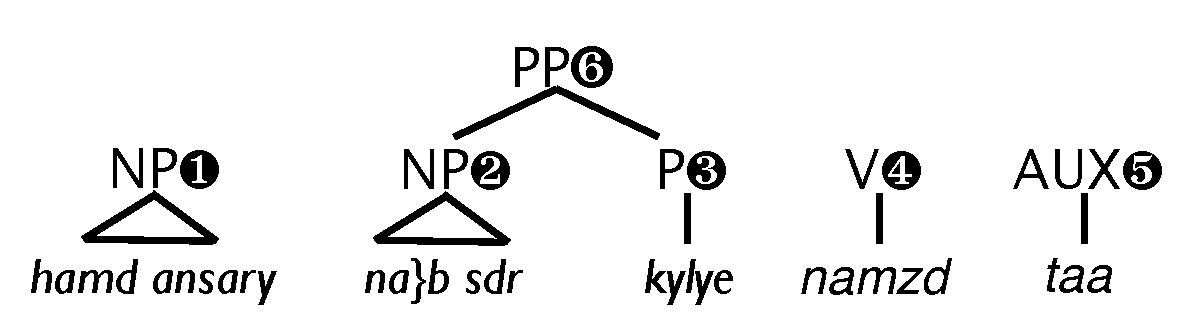
\includegraphics[width=.45\linewidth]{SCFGs/urdu-step1} & &
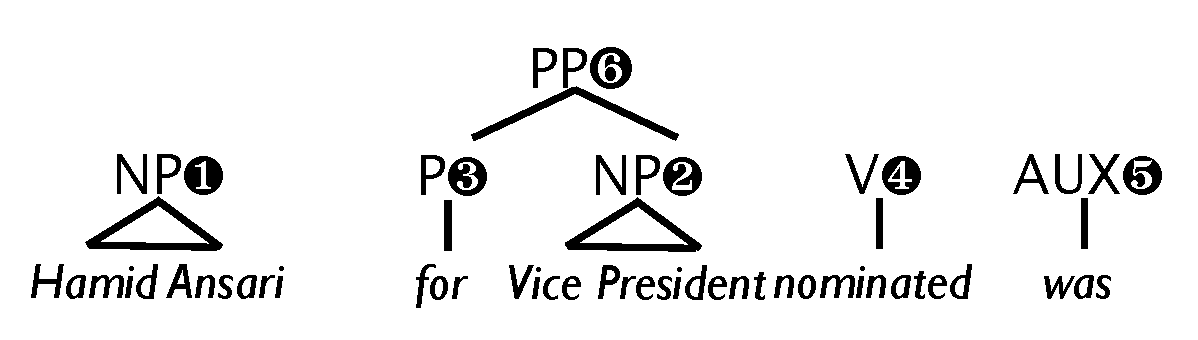
\includegraphics[width=.45\linewidth]{SCFGs/english-step1} \\ \hline\multicolumn{3}{>{\columncolor[rgb]{0.95,0.95,0.75}}c}{The English auxiliary verb and main verb get reordered with the application of the VP rule.}\\
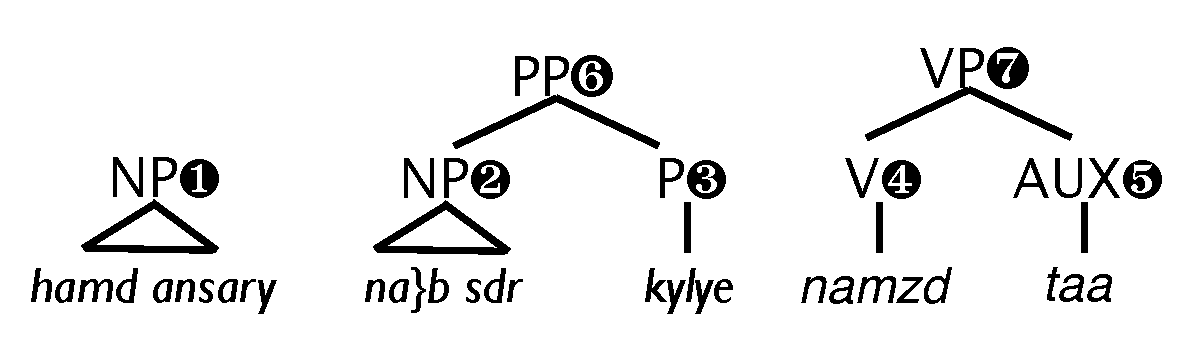
\includegraphics[width=.45\linewidth]{SCFGs/urdu-step2} & &
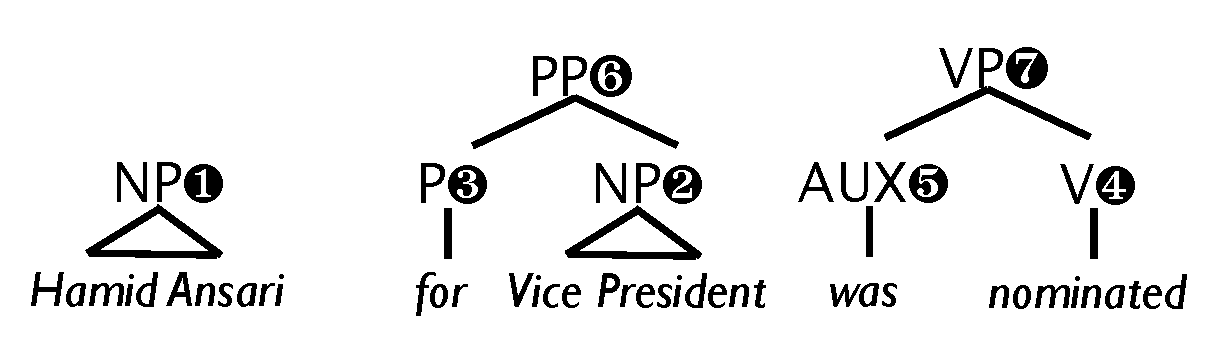
\includegraphics[width=.45\linewidth]{SCFGs/english-step2} \\ \hline 
\multicolumn{3}{>{\columncolor[rgb]{0.95,0.95,0.75}}c}{This VP rule moves the English verb from the Urdu verb-final position to its correct place before the PP.}\\
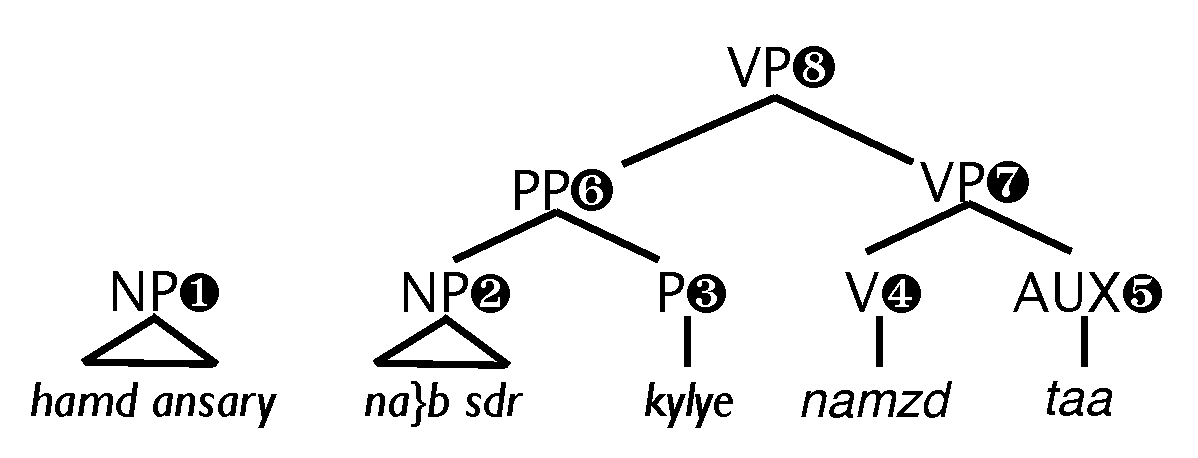
\includegraphics[width=.45\linewidth]{SCFGs/urdu-step3} &  & 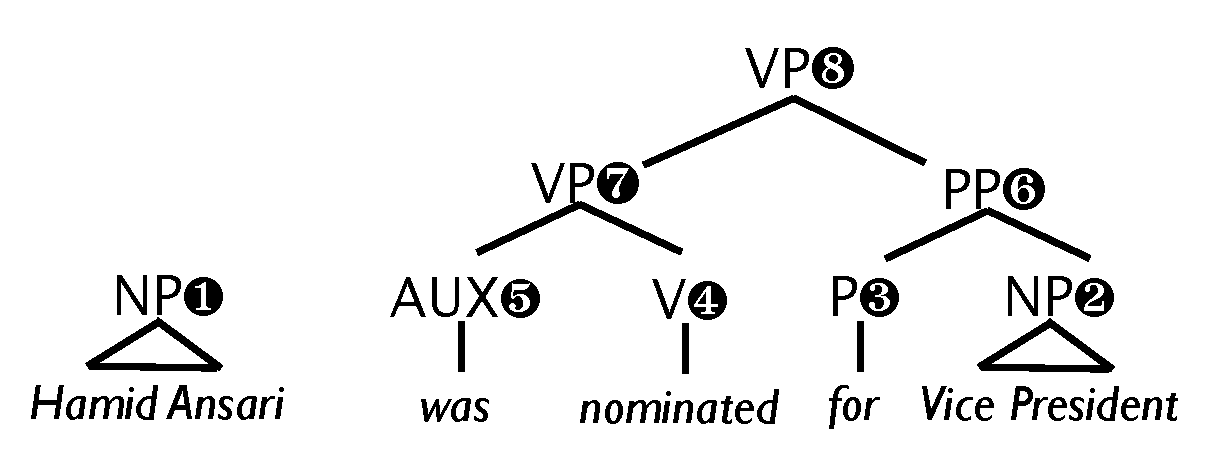
\includegraphics[width=.45\linewidth]{SCFGs/english-step3} \\ \hline
\multicolumn{3}{>{\columncolor[rgb]{0.95,0.95,0.75}}c}{Applying the S rule, means that we have a complete translation of the Urdu sentence.}\\
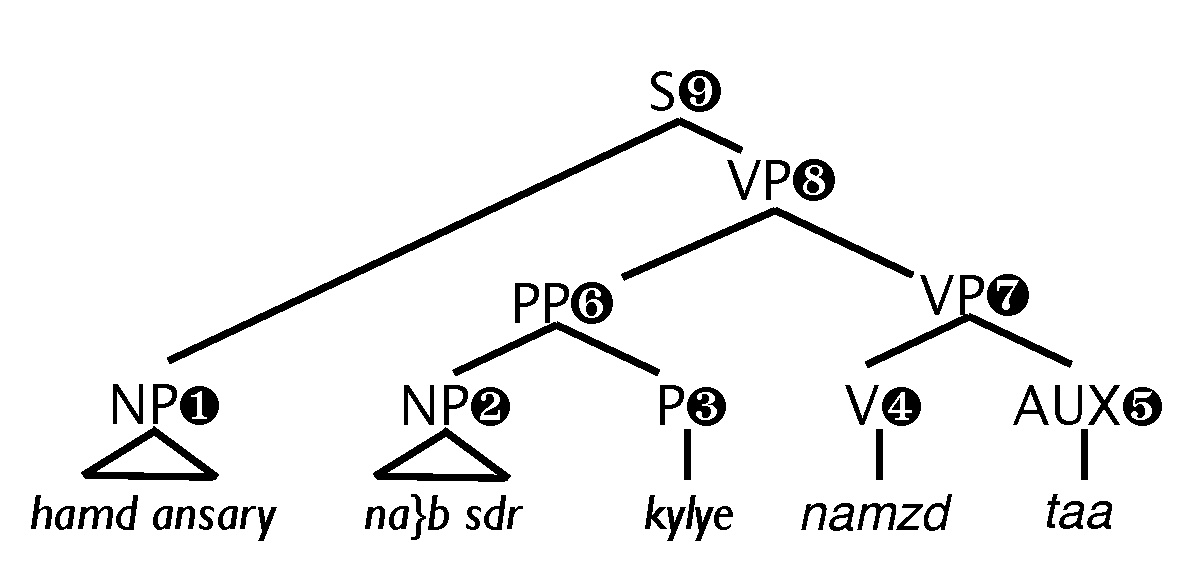
\includegraphics[width=.45\linewidth]{SCFGs/urdu-step4} &  & 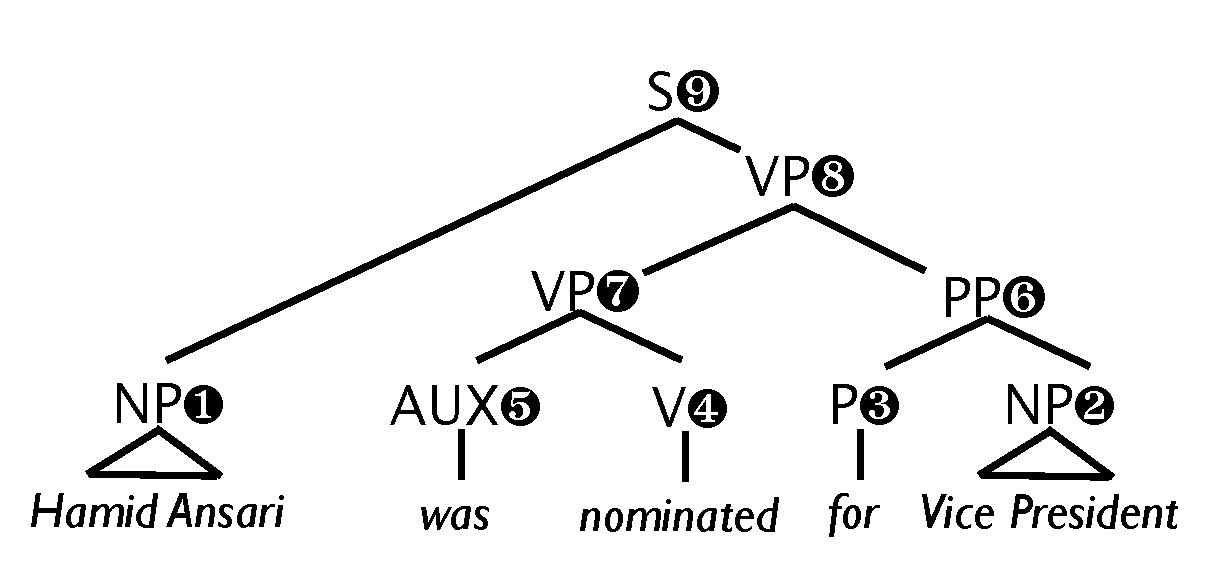
\includegraphics[width=.45\linewidth]{SCFGs/english-step4} 
\end{tabular}
\caption{Using SCFGs as the underlying formalism means that the process of translation is one of parsing.  This shows how an English sentence can be generated by parsing the Urdu sentence using the rules given in Figure \ref{toy-scfg}}\label{toy-scfg-parse} 
\end{figure}



The translation models used in this workshop are synchronous context free grammars (SCFGs).
SCFGs \cite{lewis68scfg}  generalize  context free grammars so they generate pairs of related strings.  
Because they generate pairs of strings they are useful for specifying the relationship between two languages, and can be used to describe translation and re-ordering.  
Probabilistic SCFGs can be formally defined as follows:
\begin{itemize}
\item T$_{S}$: a set of source-language terminal symbols
\item T$_{T}$: a set of target-language terminal symbols
\item N: a shared set of nonterminal symbols
\item A set of rules of the form  $\text{X} \rightarrow \langle \gamma, \alpha, \sim, w \rangle$
	\begin{itemize}
	\item X $\in$ N
	\item $\gamma$ is a sequence source terminals and non-terminals
	\item $\alpha$ is a sequence of target terminals and non-terminals
	\item $\sim$ is a one-to-one correspondence between the non-terminals in  $\gamma$  and $\alpha$
	\item $w$ is a weight or probability assigned to the rule
	\end{itemize}
\end{itemize}



A toy example of an SCFG is given in Figure \ref{toy-scfg}.  The nonterminal symbols, which are written in uppercase, are identical across the two right hand sides of the context free grammar rules, but can come in different orders. 
The process of translation is accomplished by parsing the source language input sentence and simultaneously generating the target language output sentence.  This
process is illustrated in Figure \ref{toy-scfg-parse}, which shows how parsing an  Urdu sentence generates an English translation using the toy example grammar.  The toy grammar and example parse omit the $w$ weights/probabilities assigned to the grammar rules.  In practice there are a huge number of alternative translations and derivations, and assigning probabilities allows us to choose the best translation according to the model, and to reduce the search space by expanding only the most promising partial translations. 

\subsection{Hiero: SCFGs with one non-terminal symbol}

The use of SCFGs for statistical machine translation was popularized by \citet{Chiang2005} with the introduction of the Hiero system.  Chiang's Hiero system extended the standard phrase-based approaches to statistical machine translation by allowing phrases that contain gaps.  Chiang described how these {\it hierarchical phrases} could be obtained by straightforwardly extending the standard methods \cite{Koehn2004,Koehn2003,Tillmann2003,Venugopal2003} for extracting phrase pairs from word-aligned sentence pairs.  Figure \ref{hiero-phrase-extraction} shows how a hierarchical phrase can be constructed by replacing two smaller phrase pairs with the nonterminals indexed $1$ and $2$.   These rules are written in the same format as the SCFG rules given in Figure \ref{toy-scfg}.  Although the Hiero rules are devoid of linguistic information, they are able to indicate reordering, as shown with the swapped positions of $X_1$ and $X_2$. 

\begin{figure}
\begin{center}
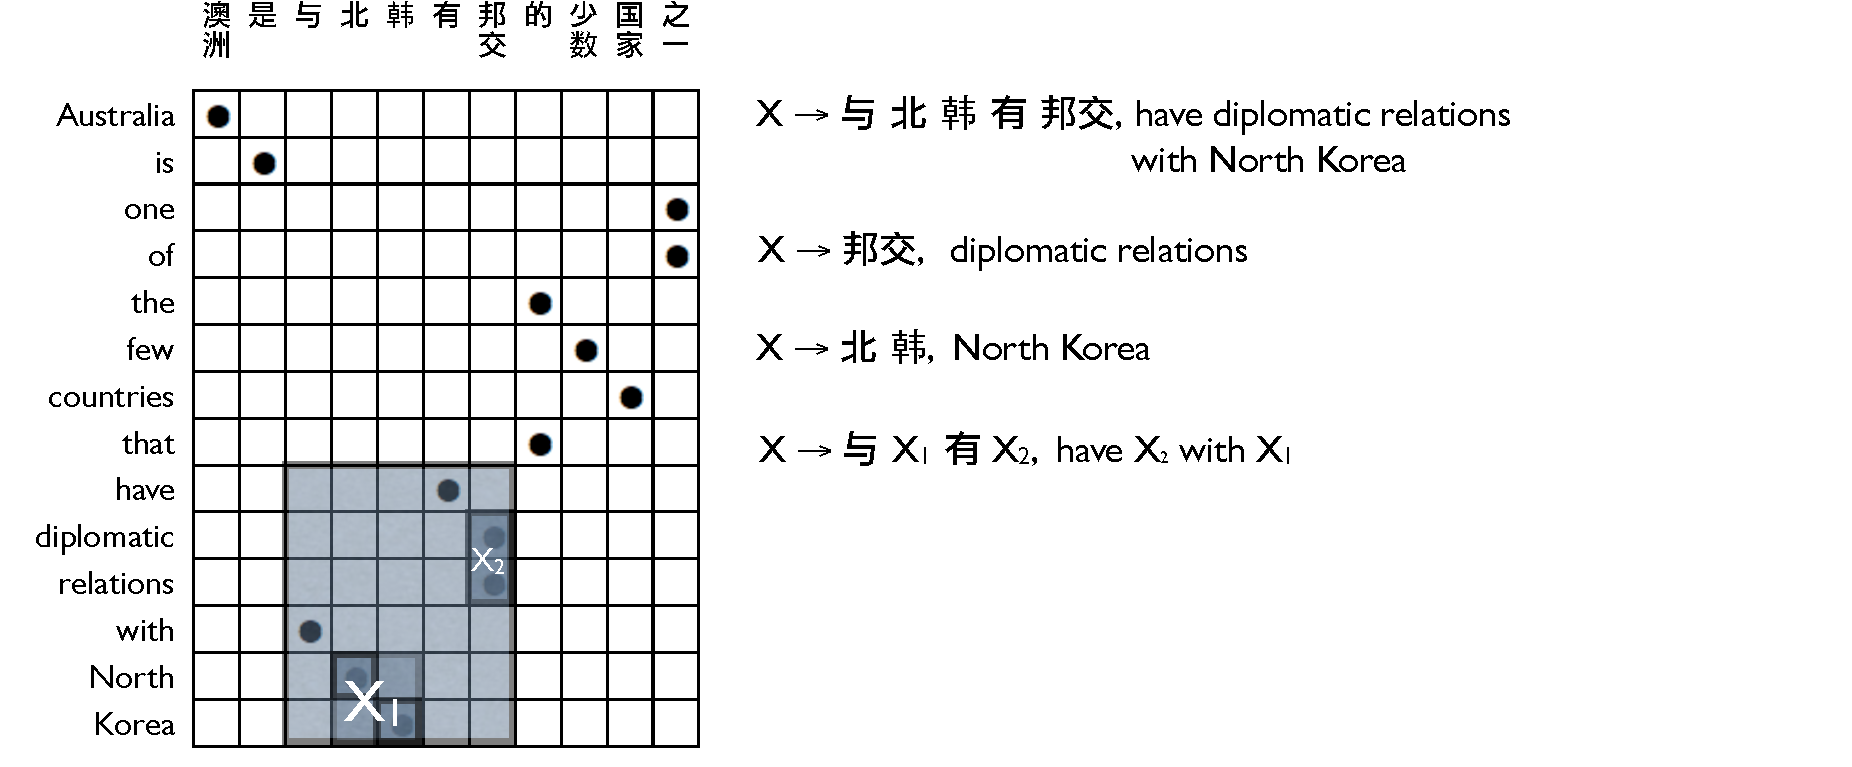
\includegraphics[width=.9\linewidth]{SCFGs/hiero-phrase-extraction.pdf}
\end{center}
\caption{An example of a hierarchal phrase extracted from a word-aligned Chinese-English sentence pair.  Chiang's Hiero system used rules that were written in the form of synchronous grammars, but which are devoid of linguistic information.}\label{hiero-phrase-extraction}
\end{figure}


Rather than using the full power of the SCFG formalism, the Hiero system instead uses a simple grammar with one non-terminal symbol, X, to extend conventional phrase-based models to allow phrases with gaps in them.  The Hiero system is technically a grammar-based approach to translation, but does not incorporate any linguistic information in its grammars.  Its process of decoding is also one of parsing, and it employs the Cocke-Kasami-Younger (CKY) dynamic programming algorithm to find the best derivation using its probabilistic grammar rules.   However, because Hiero-style parses are devoid of linguistic information, they fail to capture facts about Urdu like that it is post-positional or verb final. 

\subsection{Syntax-augmented SCFGs extracted from supervised parses}\label{samt}


\begin{figure}
\begin{center}
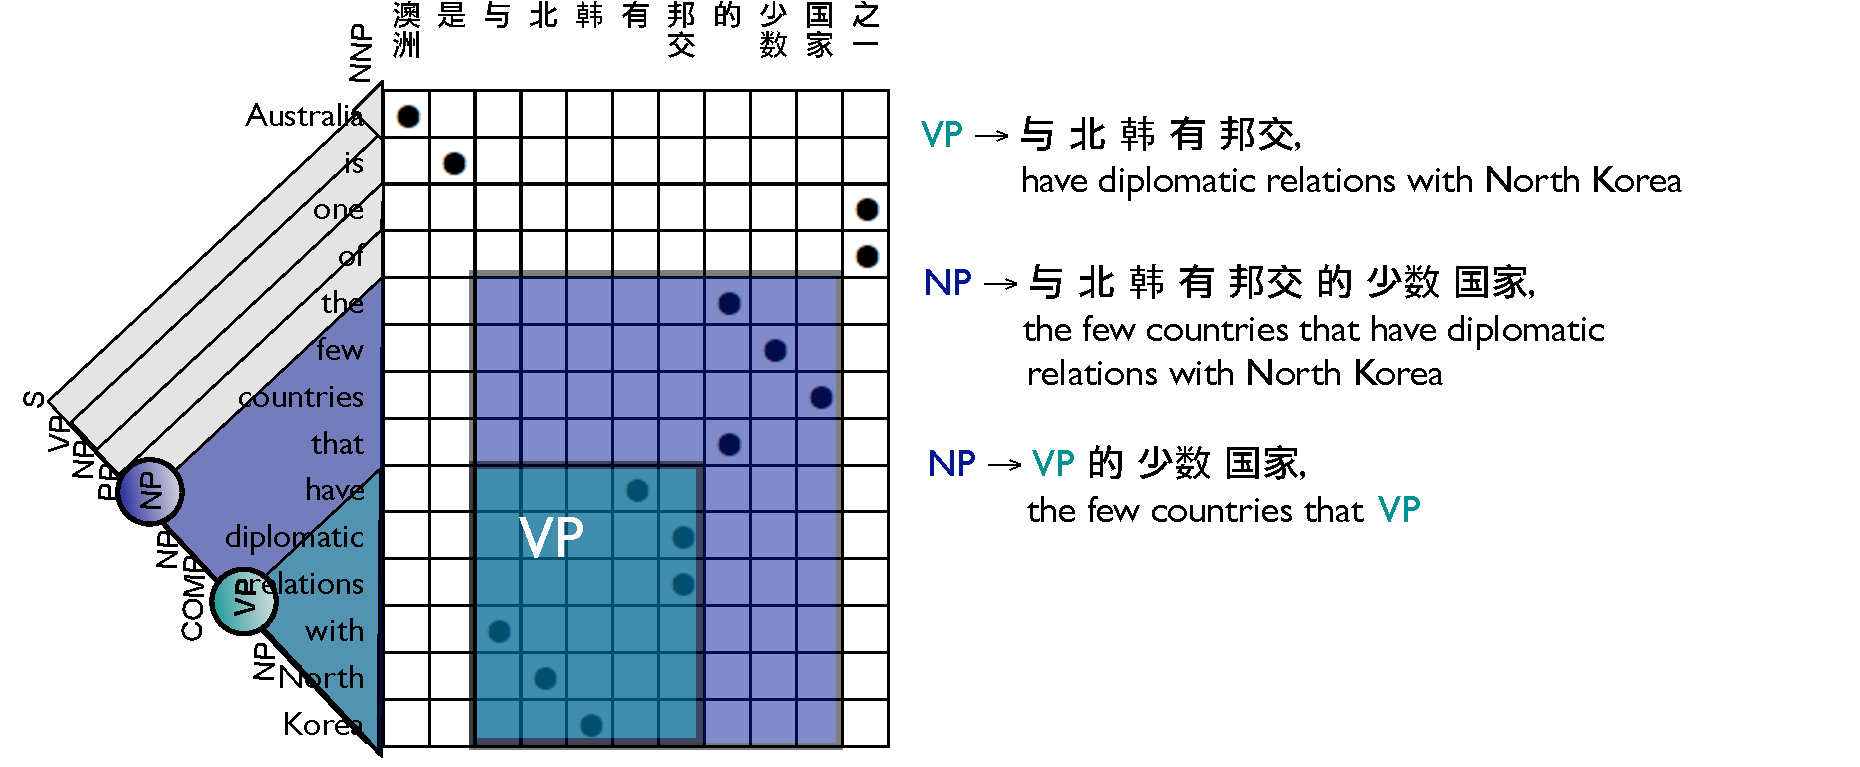
\includegraphics[height=3in]{SCFGs/scfg-phrase-extraction.pdf}
\end{center}
\caption{An example of extracting linguistically-motivated SCFGs by labeling phrase pairs using the labels of the corresponding nodes in a parse tree.  Rules with syntactic non-terminals on the right-hand sides can be formed by replacing  phrase pairs with their non-terminal labels, as shown with the VP on the right hand sides of the second NP rule.}\label{scfg-phrase-extraction}
\end{figure}


SCFGs with a rich set of linguistically motivated non-terminal symbols have been proposed as an alternative to Hiero. A number of approaches have been proposed for extracting linguistically-motivated grammars from a parsed parallel corpus \cite{Galley2004,samt}.   These approaches extract SCFGs from a parallel corpus that has been parsed using a supervised parser that was trained on a treebank.  

Figure \ref{scfg-phrase-extraction} shows how linguistically motivated grammar rules can be extracted from a training sentence pair that has been automatically parsed and word-aligned.    Instead of assigning the generic label ``X'' to all extracted phrase pairs, as the Hiero model does, linguistic labels are extracted from the parse tree.   

In the standard phrase-based and hierarchical phrase-based approaches to machine translation, many of the ``phrases'' that are used are not phrases in the sense of syntactic constituents.  They are simply sequences of words.  For example, in Figure \ref{scfg-phrase-extraction}, the phrases {\it Australia is} and {\it one of} are examples of phrases which have consistent Chinese phrase pairs, but which do not correspond to nodes in the parse tree.  If we were to limit ourselves to extracting only phrase pairs that were licensed by the parse tree and which had consistent word alignments, then we would have reduced coverage compared to Hiero.  Instead, we adopt the methodology described by\citet{samt}, which achieves the same coverage as Hiero by generating complex labels for non-consistuent phrases.  


\begin{figure}
\begin{center}
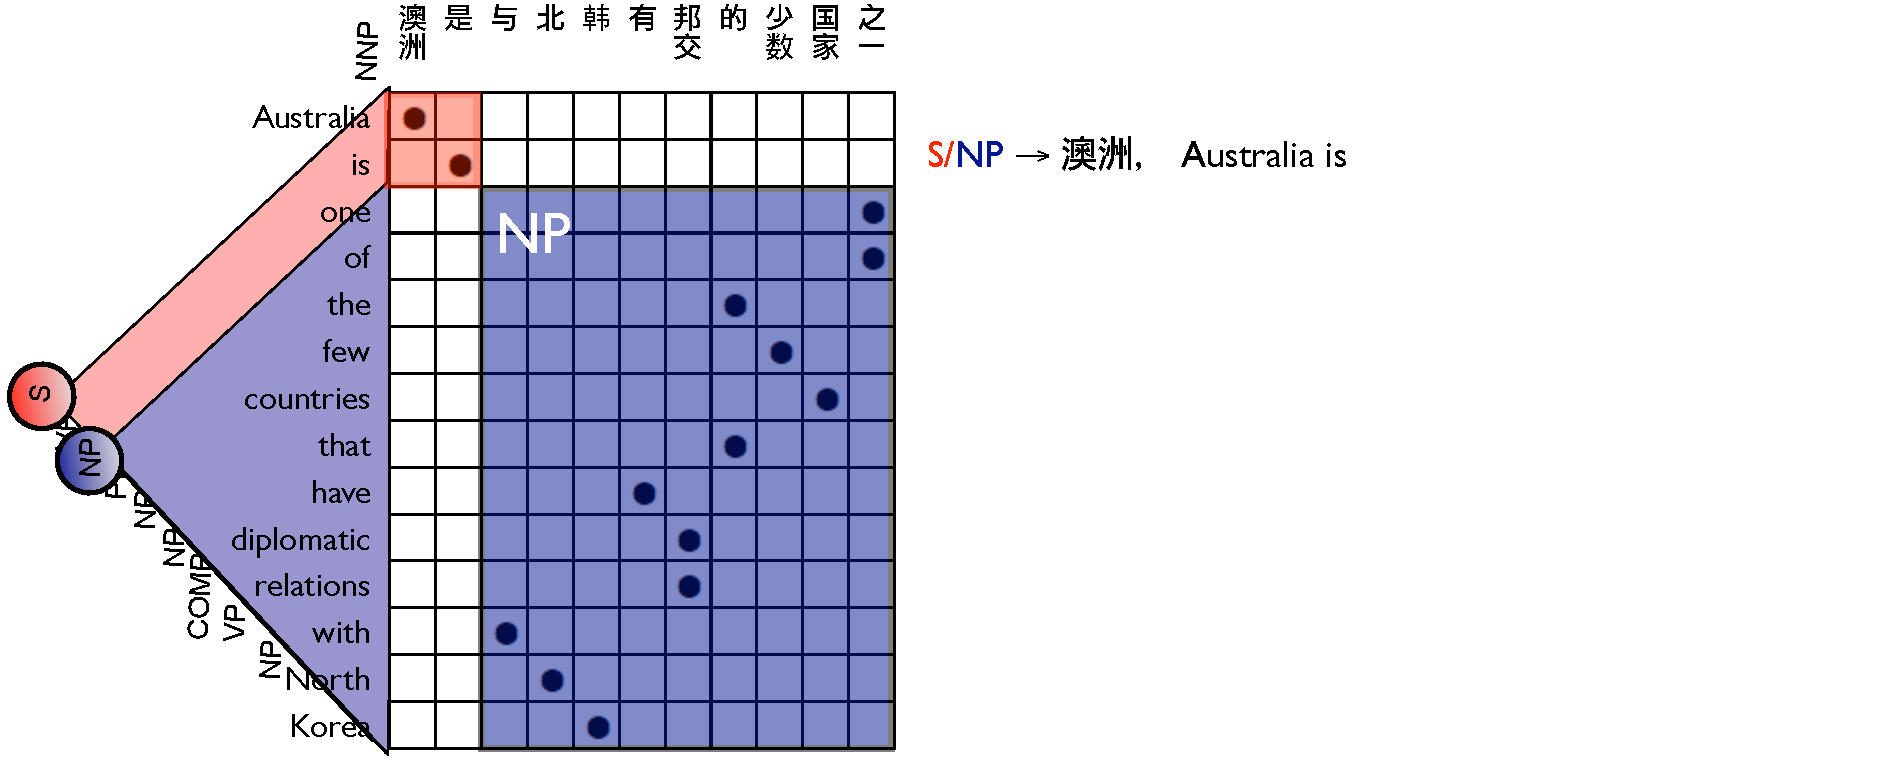
\includegraphics[height=3in]{SCFGs/scfg-ccg-phrase-extraction.pdf}
\end{center}
\caption{An example of a CCG-style label for the non-constituent phrase {\it Australia is}.  The label indicates that the non-constituent phrase would be an S if an NP were found to its right.  This complex label can be treated like any other label during parsing and translation. }\label{scfg-ccg-phrase-extraction}
\end{figure}


\citet{samt} define a framework for extracting SCFGs with linguistically motivated nonterminals from an aligned parallel corpus where one side of the parallel corpus has been parsed. The resulting context-free rules contain a rich set of nonterminal categories. These categories include traditional nonterminal categories taken directly from the monolingual parse trees (e.g. DT, NP, VP), and extended categories formed by gluing together adjacent nonterminals (e.g. NP+V, RB+JJ) and incomplete constituents that denote a category missing a child component to the left (e.g.  NP\textbackslash DT) or to the right (e.g. NP/NN) in the style of Combinatory Categorial Grammars \cite{ccg1982}.   \citet{samt}'s Syntax Augmented Machine Translation (SAMT) grammars may also include hierarchical rules and glue rules \cite{chiang:2007} that are not linguistically motivated; such rules allow partial translations to be combined (with some penalty) without regard to syntactic structure.



\begin{figure}
%\begin{center}
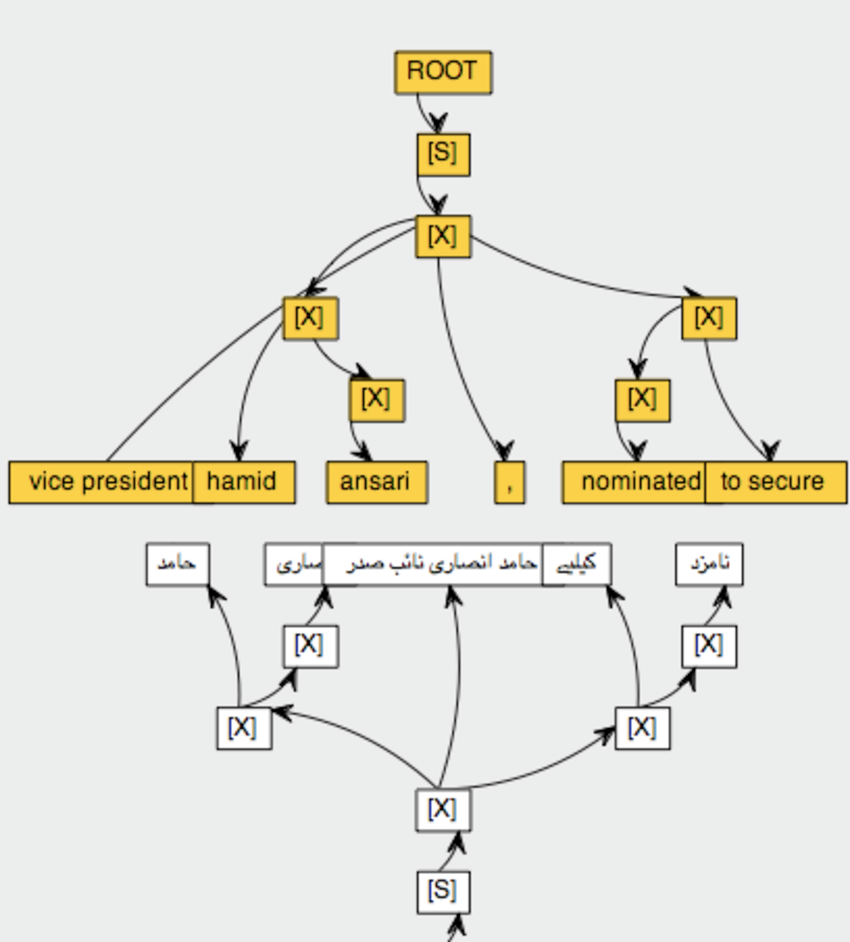
\includegraphics[height=3.75in]{SCFGs/hiero-tree}
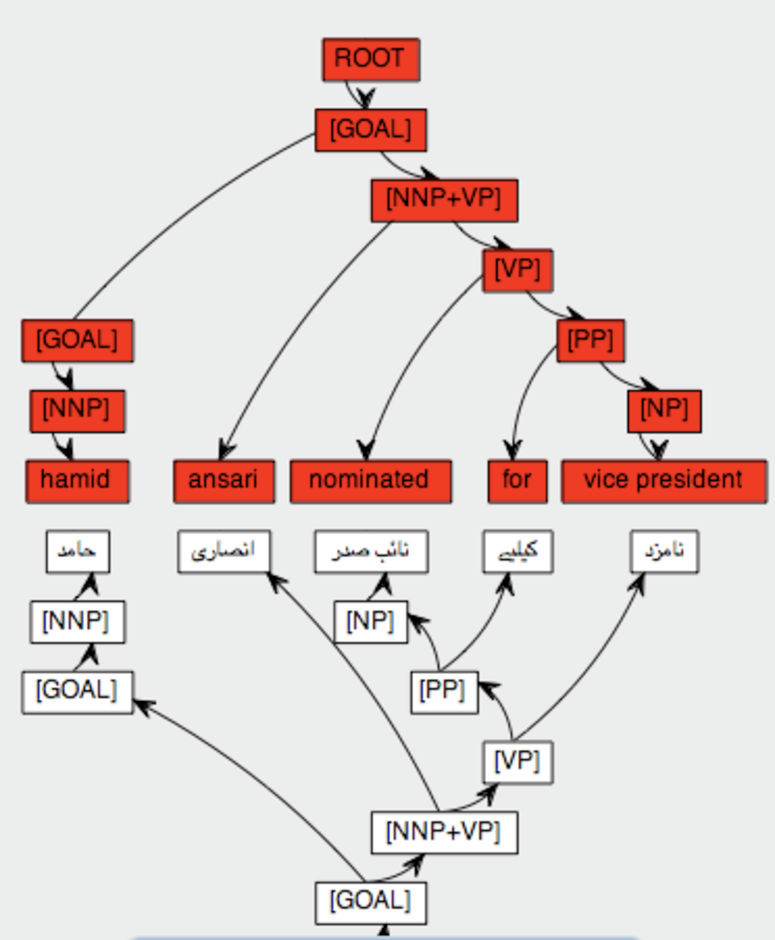
\includegraphics[height=3.75in]{SCFGs/samt-tree}
\caption{Sample derivations for an Urdu sentence translated into English translation using a hierarchical phrase-based SCFG (left) and a linguistically motivated SCFG (right).  For reference, a human translator produced ``Hamid Ansari nominated for the post of vice president" as the translation of the Urdu. }
%\end{center}
\label{example-derivations}
\end{figure}


\subsection{SCFGs with syntactic labels extracted from supervised parses}\label{samt}

Note that one of the major advantages of extracting the linguistic SCFG for an automatically parsed parallel corpus is that only one side of the parallel corpus needs to be parsed.  To extract an Urdu-English SCFG we therefore could use an English parser without the need for an Urdu parser.  During translation the Urdu input text gets parsed with the projected rules, but a stand-alone Urdu parser is never required. 
However, all of the current approaches require that a parser, trained on supervised data, exist for at least one of the languages.  

The methods explored in this summer workshop obviate the need for a supervised parser, and instead automatically induce the grammars from unlabeled texts.  The potential advantages of our approach are:
\begin{enumerate}
\item It can be applied to language pairs for which treebanks do not exist.
\item The set of non-terminal symbols is not tied to a particular treebank formalism, and therefore may be more appropriate for translation.
\end{enumerate} 


